% Created 2023-03-30 Thu 17:01
\documentclass[9pt, b5paper]{article}
\usepackage{xeCJK}
\usepackage[T1]{fontenc}
\usepackage{bera}
\usepackage[scaled]{beraserif}
\usepackage[scaled]{berasans}
\usepackage[scaled]{beramono}
\usepackage[cache=false]{minted}
\usepackage{xltxtra}
\usepackage{graphicx}
\usepackage{xcolor}
\usepackage{multirow}
\usepackage{multicol}
\usepackage{float}
\usepackage{textcomp}
\usepackage{algorithm}
\usepackage{algorithmic}
\usepackage{latexsym}
\usepackage{natbib}
\usepackage{geometry}
\geometry{left=1.2cm,right=1.2cm,top=1.5cm,bottom=1.2cm}
\usepackage[xetex,colorlinks=true,CJKbookmarks=true,linkcolor=blue,urlcolor=blue,menucolor=blue]{hyperref}
\newminted{common-lisp}{fontsize=\footnotesize} 
\author{deepwaterooo}
\date{\today}
\title{A targetted misbehavior on Propose}
\hypersetup{
  pdfkeywords={},
  pdfsubject={},
  pdfcreator={Emacs 28.2 (Org mode 8.2.7c)}}
\begin{document}

\maketitle
\tableofcontents


\section{它的个性}
\label{sec-1}
\begin{itemize}
\item 【主要目的:】摧毁一个人的名声on propose; 为的是摧毁这个人残余名声所可能带来的商业价值;以及,它个人的,从中获利,手段是:当从这个人身上打劫不到油水时,需要方方面面销毁这个人可能会对它继续打劫下一个人可能会造成或是带来的影响。
\item 【主要手段:】各种撒谎,并一直不断盖它自己的谎,以便它的谎不被揭穿,可以一直继续支持它当二房东,通过 crossing boundaries 获利。
\item 【它老板娘】
\end{itemize}
\section{三次无中生有}
\label{sec-2}
\begin{itemize}
\item \textbf{【它导师第一次带它去看WSU 女篮比赛的下午:】} 它大概因为起床晚,走得急,来不及锁门。但是它回来我问起,它谎称我早上出门时没关门,门是敞开半开状态;继而继续撒谎说我把车也开走了。。。我说我没有开车去党校,车在家里。它才认底,说它记不得我车长什么样了。我无法相信它说门上敞开半开状态,更相信它撒谎。
\item \textbf{【我第二次去COSTCO 之后一周,连续两天两次】} :制造事件,我外面打不开门,它是帮开门了,却说门没有锁,为什么我要它开门?我有哑巴吃黄莲无法对证的苦,却不知道这样的该如何继续沟通?第二天,它再说我没关好水龙头,是流水状态,无法相信,感觉自己的智商情商被愚弄,它是想要对我证傻?
\end{itemize}
\section{主要 scheduling}
\label{sec-3}
\begin{itemize}
\item \textbf{【租住时:我方】} 原计划是两个月,差不多是到 3/31/2023.
\item \textbf{【租住时:它方】} 它隐身暗处的做法是,找时机,适时清楚清晰告诉你:它的工资是由它自己的国家土耳其支付,它不领领不到WSU 任何工资。让你清楚感知,正如它的招租贴子在网上,它有经济帮助需求, \textbf{我同样想要去帮助它。心理上,我也从来觉得我们互相帮助,两个人平等。}
\item \textbf{【过程中,WSU EECS Ph.D Application ※ Admission:】} 因为申请Ph.d in EECS, waiting for result, and unofficial admission. Boundaries did have been changed from my side, but I have always notified her the first time I could, and I think she is notified and clear about all the changes, and I have NEVER expected her ABNOMAL BEHAVIROS. 
\begin{itemize}
\item Submitted Application time: around 1/30/2023?check
\item \textbf{Unoffical admission time: 3/2/2023}. I stated I would wait for my official admission so that I may be qualified or they may be able to consider my applying for residence for Spring and Summer semester. She did NOT refuse, nor stated anything. \textbf{【Boundaries did have been crossed from my side as I was happy for my admission, and proud to be a coug.】}  But she knew it, and seemed she had no problem with it at all. No refuse from her side.
\end{itemize}
\end{itemize}

\section{租住过程中的主要事件与日期设置}
\label{sec-4}
\begin{itemize}
\item 3/1/2023: When I paid the monthly rent that day, I checked her required notice time, she answered 2 weeks. I stated I will make sure I leave her at least 2 week notice time.
\item \textbf{Unoffical admission time: 3/2/2023}. I stated I would wait for my official admission so that I may be qualified or they may be able to consider my applying for residence for Spring and Summer semester. She did NOT refuse, nor stated anything. \textbf{【Boundaries did have been crossed from my side as I was happy for my admission, and proud to be a coug.】} But she knew it, and seemed she had no problem with it at all. No refuse from her side.
\item \textbf{3/7/2023}: She set hard deadline from her side that her boyfriend is coming for visiting her in May. My last day of staying with her would be 5/1/2023.
\end{itemize}

\section{当事件结果不如预期,个性上,它傾向于首先去怪罪别人}
\label{sec-5}
\begin{itemize}
\item \textbf{【吃饭小费问题:】} 周日,它因为不愿意出小费,而语言上攻击怪罪我,强说我迫它出去吃的!!!我狠无语。
\item \textbf{【第二次 COSTCO 两样东西:】} 它两面三刀怪别人逼它买,我没有。它至少有两次非常清楚的选择、自主作决定机会. 周日跟它清楚解释过,它承认了我没有逼它。
\end{itemize}

\section{三次 article-shock 想法撞击}
\label{sec-6}
\subsection{Recommendation for EECS Ph.D Candicate}
\label{sec-6-1}

\includegraphics[width=.9\linewidth]{./pic/readme2_20230329_114352.png}
\begin{itemize}
\item I felt it was very cold, a Recommendation letter from some person 10000 miles away. did feel shock. But communicate and adjusted to be:
\end{itemize}

\includegraphics[width=.9\linewidth]{./pic/readme2_20230329_092732.png}
\subsection{Suggestion for replying back a potential Ph.D Candidate screening from my advisor}
\label{sec-6-2}
\begin{itemize}
\item 收到邮件那天晚上,它要看我的邮件,我就让它看。它口头表达困难,但写,却可以极端清晰地表达出它的观点:因为重点分明,言简意该,清楚地知道如何选择角度与用词来表达支持它的立场,没有任何废话。
\item 使用 google translate: 它的观点清晰可见:我从13 年到现在九年工作了(只有)五份工作,是个彻底的 LOSER. 它非常个人偏见地,把别人的录取扫描偏见成为其它它并不真心 appreciate 它所工作的单位的方式。
\item 没有纪录,无法追塑。【这更像是一个人摧残别人正常三观与价值观的方式,非常人能表达如此观点。。。】
\item 被它的观点,被它心底我是一个彻头彻尾的雷到外蕉里嫩,像一盆液氮沷在身上,彻底被 shock, 希望一秒内结束与它所有一切的谈话,再无任何想要跟它继续讨论或是说的话。
\end{itemize}
\subsection{昨天的它提供的它的说词:我同样被它一再的撒谎与,它所选择的撒谎、角度与用词表达,雷到}
\label{sec-6-3}
\begin{itemize}
\item As we confirmed and cleared in front of the policemans, that we do NOT need to help the other, I believe we should take our full financial responsibilities towards the mistakes we made earlier. I do NOT need your help, and you can always take your full financial responsibilities as well then you are trying to help any other person.
\item I did NOT see any paper document on dining table last night.
\item If you do have it ready, please leave a copy on the dining table before you leave for office today, so that I could bring it with me when I consult for professional advise considering my international background, as well as you first four months international cultural shock in US. And they may be able to offer more exact suggestions how I should handle this case. Thank you.
\end{itemize}

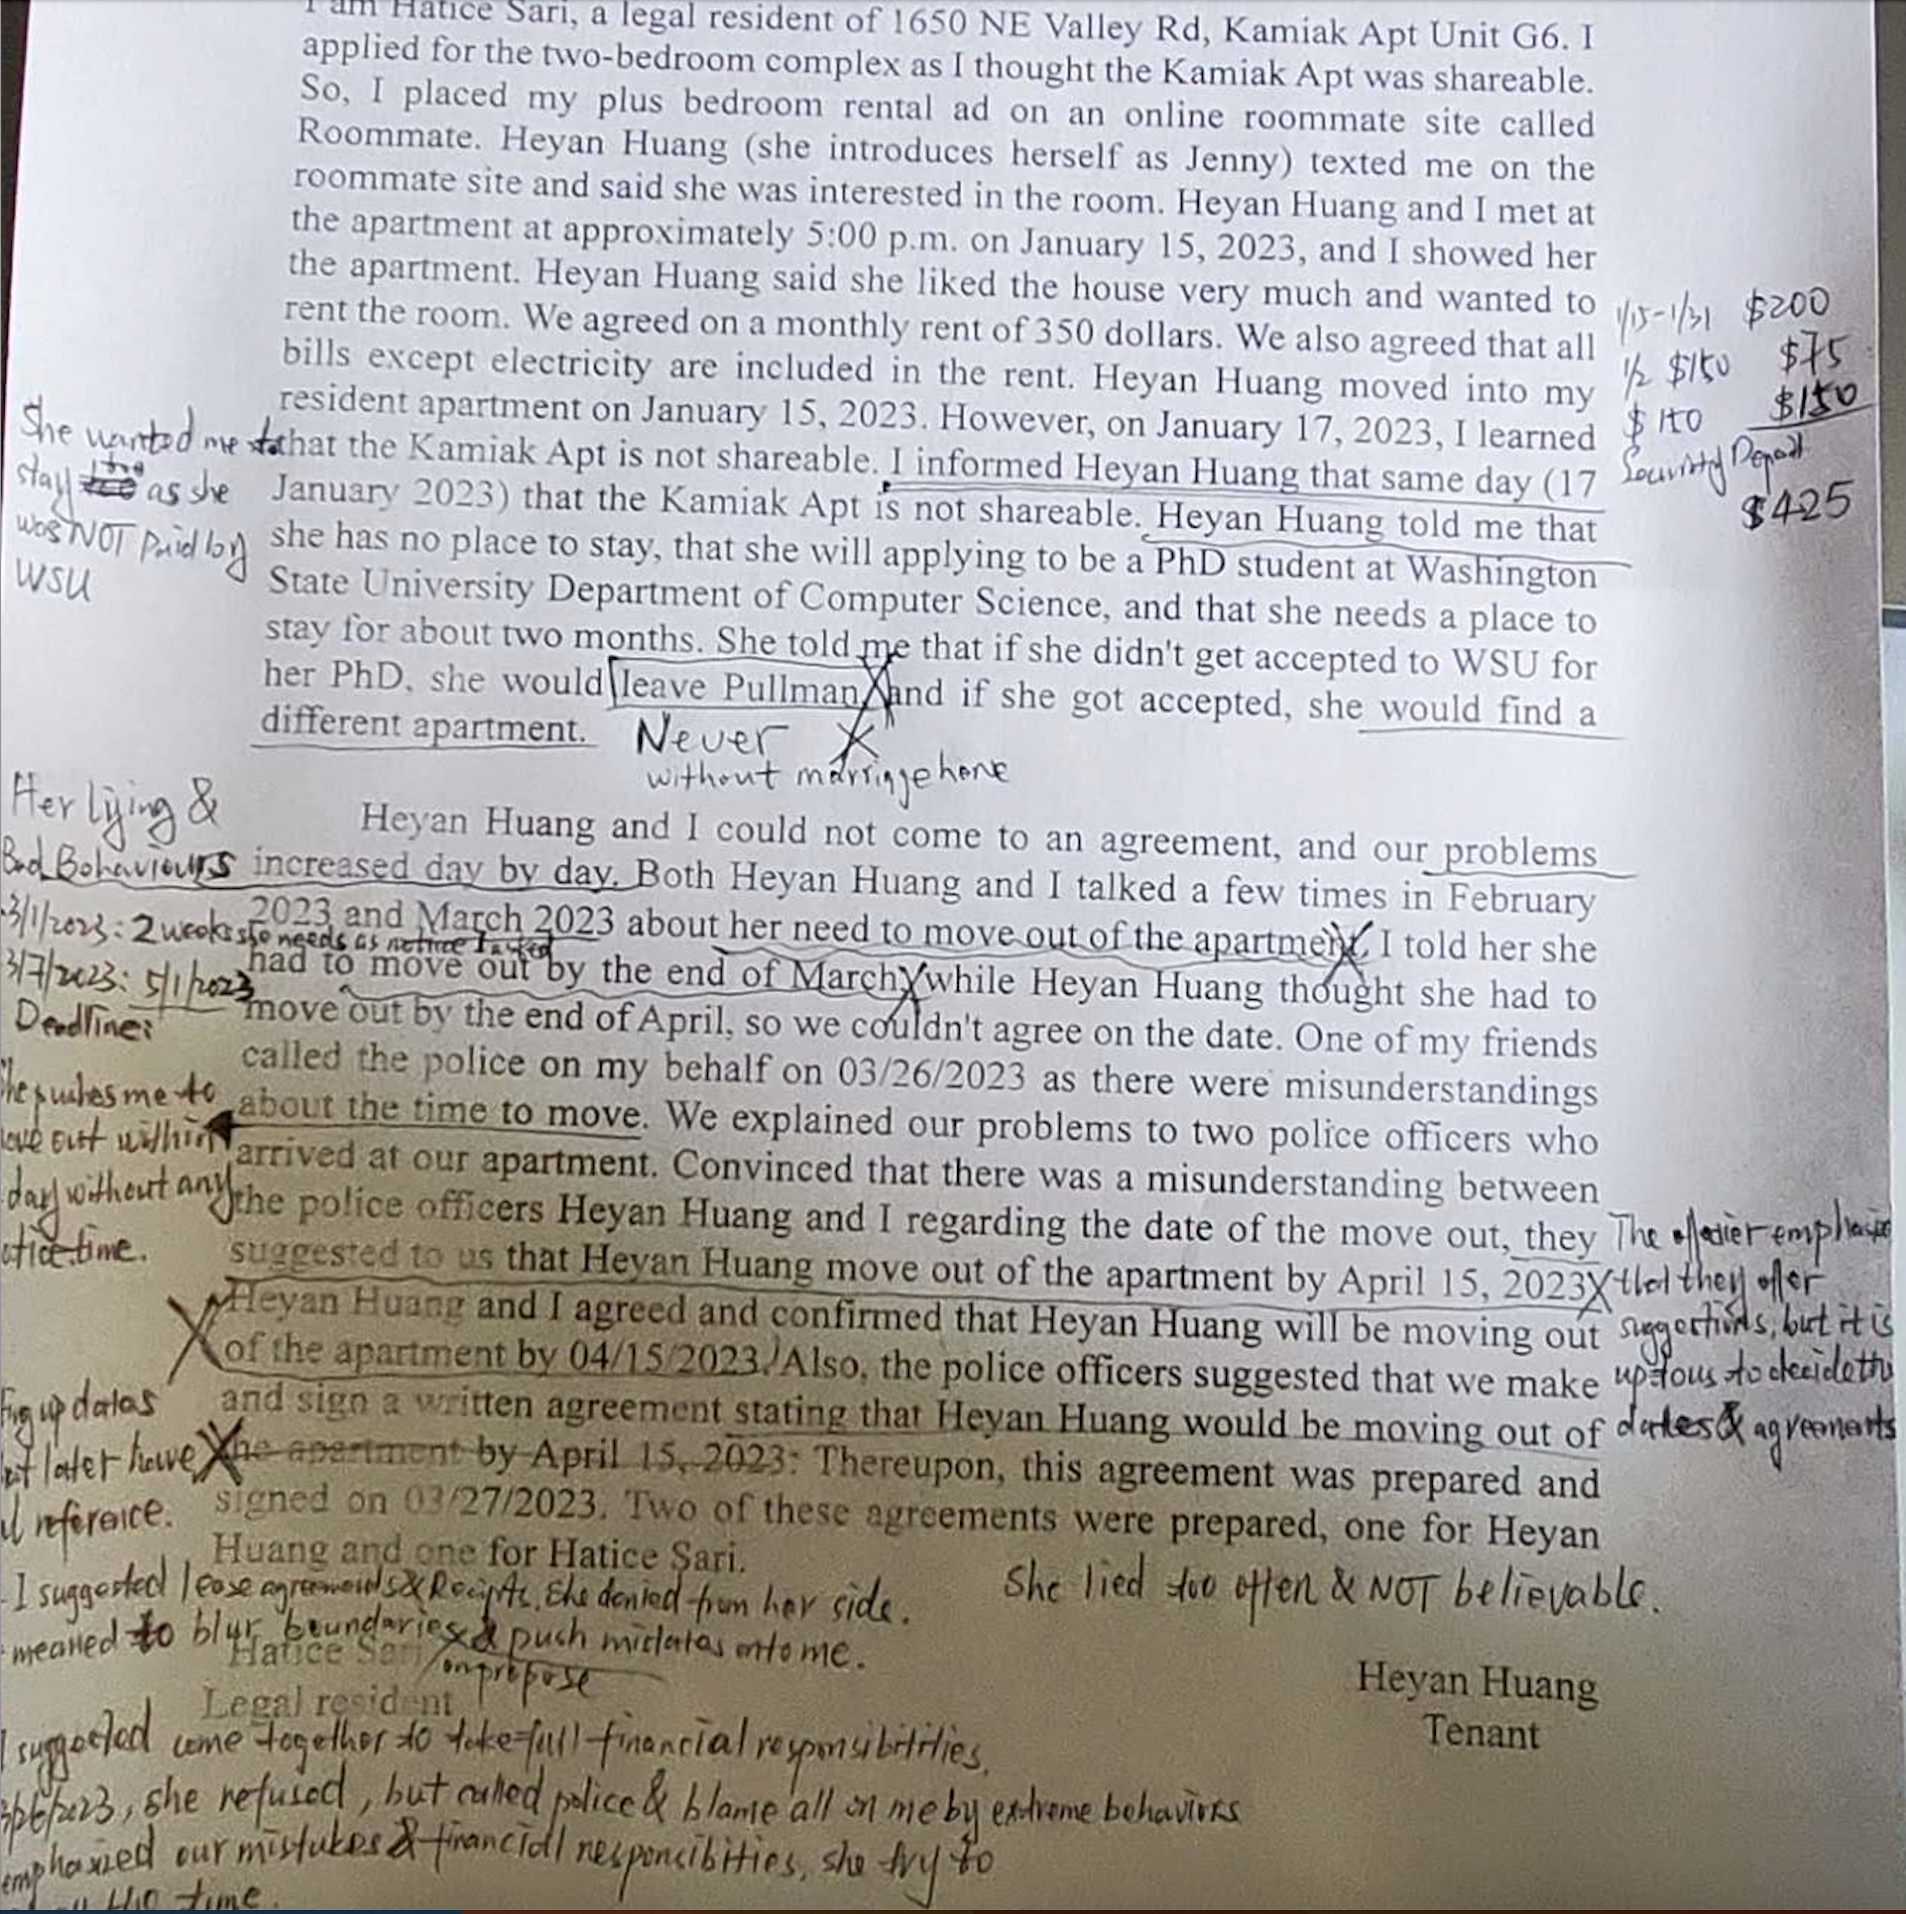
\includegraphics[width=.9\linewidth]{./pic/readme2_20230329_102715.png}
\begin{itemize}
\item \textbf{【这个人故意制造事端,并不曾有任何真诚交流沟通:】} 当我第二次去COSTCO 它付我 \$8 块钱油费(\$36 一月电费账单包括了36 天,我 15 号晚上入住),它还想用总共2.27 两样东西代替而它想不通周六晚上在它自己床上咳呈咳时,我周日傍晚,(因为两个国际人)拿笔拿本在厨房餐桌上与它花费大半个小时帮它一一解释清楚。
\item 而它,对待它的室友,除了制造各种极端,没有半点真诚与努力,而是故意制造极端事件,制造事端。
\end{itemize}
\subsubsection{这里,就看出出问题的主要点在:}
\label{sec-6-3-1}

\includegraphics[width=.9\linewidth]{./pic/readme2_20230330_164636.png}
\begin{itemize}
\item 我一直以为当它说它误以为我3/1 交她房租时,它说我3/1 号说过我要 3/31/2023 搬出去。我给她更正,我3/1 号交房租那天,我表达的是我想要在月底能够搬出去,我并没有说一定能够3/31 就搬出去。我说过,一旦我找到住处,我一定会 make sure 我给它留两周 notice 时间。这个样子记忆里大概也就发生过一两次。因为紧接着收到非正式录取,我就跟它表达了我想等正式通知下来。它仍然是没有话。
\item 这里说成为,它不说话,我总以为我给它更正过,或是表达过,通知到它,它没有提任何反对意见,便是默认了。
\item 这里,它作为一个初到者,听力可能不够,语言表达可能不够。但它真的狠能够写,可以看成个思想评论家写手枪手。
\item 我们之间,我有意识到最近它越来越故意吵别人休息的问题,但我从来没有意识到它心底还埋着这样的雷?因为它无声无息,让你完全意识不到问题的存在。
\end{itemize}
\begin{minted}[fontsize=\scriptsize,linenos=false]{text}
亲爱的表哥
活宝妹觉得事情到这个份上
其实真的摆得狠明白
就是这个室友的 blackmail 你活宝妹的 personality
不管是它头 4 个月呆美国的 cultural shock

当你的活宝妹可以付出时间精力帮助它解释清楚
对它真诚道歉说
It was my fault that I own you an explain why yesterday I accepted your wavor of my Jan utility part comfortably.
它的 1 月份我的电费部分$8.5
我为什么能够坦然地接受
我帮它画了 5 页给,给它一点一滴地解释清楚

但它 cross boundaries on propose
你的活宝妹觉得通知到它,它看起来没有问题,一切看起来似乎都没有问题

它如这个写的里面,认为是日益增长的问题
它的口语表达是差狠多,但它狠会写,写得从来都精确到位

但它却故意,甚至没能让你活宝妹意识到,两人之间存在这个问题
这个边界,被它人为拖延,又及时暴力发威,狠过分!!!

没有纸,没有笔,没有任何先前的哪怕相对 formal 的 text message
or any email emphasize

它直接来个暴力911 来暴力打劫你活宝妹的 personality
真的是狠过分

活宝妹觉得它,欠你活宝妹一个真诚的道歉
道歉的内容哪怕只是一个国际初到者,处理方式不当
深深地伤害了你活宝妹。。。。。

爱表哥,爱生活!!!
活宝妹就是一定要嫁给亲爱的表哥
爱表哥,爱生活!!!
\end{minted}

\begin{itemize}
\item 其它写过的它撒谎的角度
\end{itemize}
\begin{minted}[fontsize=\scriptsize,linenos=false]{text}
亲爱的表哥
有一点儿想到还是狠想笑:

亲爱的表哥
全世界都知道:
活宝妹若是还没能嫁给亲爱的表哥
活宝妹就是永远也不会离开亲爱的表哥所在的小镇半步

为什么,这个人哪怕是撒谎
也一定要编出个:
if she didn't get accepted to WSU for her PhD, she would LEAAVE PULLMAN
你的活宝妹永远也说不出上面的话

可是
亲爱的表哥
全世界都知道:
活宝妹若是还没能嫁给亲爱的表哥
活宝妹就是永远也不会离开亲爱的表哥所在的小镇半步
为什么,它撒谎,也一定要编别人会离开?

想起来,感觉真是好笑
人在某些方面,某个题材,比如感情爱情相关主题上的思维模式不同,处理能力方式不同
人与人之间,差异好大


亲爱的表哥

活宝妹就是一定要嫁给亲爱的表哥
活宝妹就是一定要嫁给亲爱的表哥
活宝妹就是一定要嫁给亲爱的表哥!!!

重要的事情说三遍

活宝妹嫁给亲爱的表哥了
活宝妹是个亲爱的表哥控
活宝妹嫁给亲爱的表哥了
就所有的一切,亲爱的表哥说了算,亲爱的表哥,说什么算什么!!!

可是活宝妹若是还没能嫁给亲爱的表哥
活宝妹就永远守候在亲爱的表哥的身边
活宝妹会永远守候在亲爱的表哥的身边
活宝妹会从此再也不离开亲爱的表哥的身边半步

爱表哥,爱生活!!!
活宝妹就是一定要嫁给亲爱的表哥
爱表哥,爱生活!!!
\end{minted}

\section{Boundaries have been confused and crossed by her all the time}
\label{sec-7}
\begin{itemize}
\item \textbf{1/15/2023, 1/17/2023}: when deciding accepting me renting here or not, \textbf{boundaries have been crossed on propose} known to both of us, as both of us think the other has needs and need some help. I did ask what if the administration department asked, she answered that she would admit that I was/am her girlfriend.
\item \textbf{【第一次带它出去买菜:】} 用一盒最大包装的蓝霉试探。我帮它,带它出去买菜, 给它方便出去买菜的机会;它那里怎么就变成了,它陪我出去买菜,它只要一盒最大包装的蓝霉,变成了我得付一盒蓝霉的钱,来感谢它陪我出来买菜???它试图 take ADVANTAGE OF ME. 【第一次,可以当作两个人共同,或是沟通的问题】
\item 但是后来就会发现,这个人故意各种搅和边界。每次出去,说5 分钟之内我们出去,怕是 15 分钟看能否出门,最长一次整过一两个小时之后。极其烦人。
\item \textbf{【搅和边界:它私自推开过我的房间门】} 。我第二天傍晚回家提醒它:没有我的允许,它不可以开我的房间门。
\item 【第二次 COSTCO 两样东西:】它两面三刀怪别人逼它买,我没有。它至少有两次非常清楚的选择、自主作决定机会
\item \textbf{【过程中,WSU EECS Ph.D Application ※ Admission:】} 因为申请Ph.d in EECS, waiting for result, and unofficial admission. Boundaries did have been changed from my side, but always notified her first time, and I think she is notified and clear, NEVER expected her ABNOMAL BEHAVIROS.
\end{itemize}

\section{Stated communication helps Suggestions}
\label{sec-8}
I did NOT realize that you took apartment key with you until a moment ago when I was planning go out for biking. I understand and agree that it is hard for both of us to talk to the other by us own nowadays. 

But I don't think you are supposed to bring key away and limit my access of using it. 

You tried your options of bring your friends, and called police yesterday. I agree with them that we need to set up and sign paperwork to legally protect ourselves, even before you had denied this suggestion. 

If you are not referencing their suggestions, my current out of mind ideas include the following: 

\begin{itemize}
\item appearantly it was both of our mistake trying to help the other. No need, and we could admit our mistakes to apartment administator, and conpensate financially from both of us for our bad influence on compus, as well as tear out damages.

\item I will consult info about availabe sharable apartment. And if they do have, I will try to move out as soon as possible.

\item As we may be sufferding from talking to each other by us own, it may be a good idea reach out for help from them -- the current apartment administator. They are the resource that we could try to reach, and help ourselves out.

\item Othewise, if not needed by you, I still prefer help from administatation department to solve this without abnormal behaviors. By which I mean, at least a third person resource as evidence, instead of talking between us. I prefer set up deadline of 4/30/2023. But we need setup paperwork as soon as possible, so that later you could take legal action if I am doing anything wrong.

\item Please return my car key tonight, and I don't feel safe leaving it with you any more.

\item I am currently staying inside the house, not knowing if I am able to leave the door unlocked. as no known knowledge about your opinion.

\item If you agree we reach help from apartment administator, I will try to adjust to your schedule for meeting them, when you are availabe recently.
\end{itemize}

Thanks for your attention. And I appreciate 。。。

\section{Stated lies she made earlier}
\label{sec-9}
\begin{itemize}
\item I was sitting inside the house, the apartment administration officer outside, asking if she smoke inside the house. She did. But she did answer she smoked outside and her cloth had some leftover smells. [before spring break]
\item She hidenly expressed her needs by stating she is NOT paid by WSU, but by her own country and government, which did make me feel she is in need of help at same time.
\item I suggested lease and receipts initially, she denied to avoid all possible troubles. And suggested and saw me deleted my asking for receipt text message.
\item Meanswhile, she crossed all the boundaries to be in favor of herself all the time: 
\begin{itemize}
\item 3/1/2023, I checked with her about her required notice time, she stated 2 weeks. I said I will make sure I give her 2 weeks notice time. But she blured and pretended to misunderstood the communication and stated I claimed to move out on 3/31/2023 but I did NOT.
\end{itemize}
\item I did have been waiting for my Ph.D admission. And after I got unoffice one, she and I changed the deadline together by waiting for my formal admision so that maybe I could apply for WSU sharable housing for spring and summer semester as a formal Fall 2023 Ph.D student.
\item The day I got unformally admited, I expressed my wish of after having been formal admitted, I want to apply for sharable housing. She did NOT really have any tear, but she pretended she has tears to wipe, and she did wipe her eyes, and made me think she is still in need of my help for her to afford the rent.
\item On 3/26/2023, she tried extrema behaviors towards me without any chance, as she on propose all the time lied to pretend her stand:
\begin{itemize}
\item I suggested my turn of chance get understand by her, as she has at least apologized to me once, she denied;
\item I suggested 5 days is not enough for urgent notice, if not allowing time, allow some finacial compensate, she denied;
\item I suggested the finacial compensate may not apply on me, but return back to WSU as we did break the rules, she and all her friends denied. She does NOT want to take any responsiblity on her proposed breaking the rules.
\end{itemize}
\item Yesterday I suggested, emphasized these to her too, but she ignored them on propose to financially protect herself, but blame all mistakes on me.
\item she LIES ALL THE TIMES ON PROPOSE.
\item She does NOT offer any formal discussion with me, nor bring any emphasized text message, nor any effort on such a matter, but rather, by casting a significant scene of locking me outside the house without previous
\end{itemize}


\section{心机女的故意设置背景}
\label{sec-10}
\begin{minted}[fontsize=\scriptsize,linenos=false]{text}
亲爱的表哥
你的活宝妹刚才出去骑车,终于想明白了狠多事

关于昨天晚上的钥匙,我车的钥匙
车的停车位
与家门的钥匙
我昨天 emphasized-and-notify 它的
关于我今天会去反馈承认自己做错过的事

实则,仍是如那个周六晚它不想付我 1 月份 $8 电费
先几天前终于大方一次假惺惺送一个 1 块的汉堡
再周六晚假装买错,送个 1.17 的 pizza
再说它要两样东西,付你它该付的 $10
再紧接着跟你提:1 月的电费,它说它算的是我的是 $10 钱
它帮我 wave 掉,当作我车的油费

亲爱的表哥
你的活宝妹呵呵傻傻地答应过
但当天晚上它躲它房间的咳嗽让我觉得它似简想不通
意识到这点儿
活宝妹觉得当别人请过它吃饭,它不付小费不说
接着别人帮它带它买菜,它还要用一盒最大包装的蓝霉继续试探
活宝妹觉得它的试探本身,已经伤害了别人的善意
所以接着的第二天傍晚,跟它解释清楚明白
我没有想要占它什么便宜
我会尽力帮它,也希望它能够平等待我

亲爱的表哥,你知道吗
到今天傍晚之前,你的活宝妹仍是傻的
因为傻的人今天之前都不明白:

如它这般作了国际贱鸡,打着打劫别人如意算盘的人
在你活宝妹任何想当然地以为是应该的时候
在它国际贱鸡眼里,从来都是不应该的

当你活宝妹觉得1/17 它决定租房给你活宝妹住
它就应该平等地待你活宝妹的时候
在国际贱鸡,从一开始就直接租住2 bedroom 来谋财路的人眼里
从来就不公平的:因为别人原本就是坐定高高在上二房东位
原本就是来以二房东之位来打劫财路的
你想公平?你好傻好天真。。。。。

当你活宝妹给它解释了那些
它内心底极端失望,不方便明白
却故意间接发沷发疯以退为进猛攻
你的活宝妹仍是不明白

你的活宝妹觉得 350 房租出了一半
跟它我不搞什么我住小房间少出 20 块之类的事
希望它平待待你活宝妹的时候
想要谋财的国际贱鸡,心高气傲,眼里从来不止这点儿
它想谋要财路呀,你活宝妹尽只这点儿油水儿?!!!

亲爱的表哥,它冒着二房东做案的风险
永远想要打劫更多
想要别人一天三餐做饭给它吃
可惜鱼里想加两个鸡蛋时,它的拒绝:
它这天吃过两个鸡蛋了,我只加自己的就可以了

亲爱的表哥,当你活宝妹想到,
它若是主动提它愿意出个鸡蛋送人活宝妹吃你活宝妹一定狠开心
但正如它 $6.95 精确到分归还你活宝妹会失望
当它拒绝再多一句,你的活宝妹也会去想
当它发疯时说,所有的好只有一餐饭,是如何抹平的?
就是我出鱼它出面,两个人便是平等的如此抹平的
你的劳力,在你眼里,是劳力奉献
在它眼里,是你久它的,真的,因为它量你市面上找不到这个房价的房间
而它,也就是用 350 的房租作幌子
真心实在想要打劫压炸油水来的。。。无耐成熟姜老,油水太少,它打劫不到

怎么办呢》?打劫不到油水就打劫劳力呀
它不再倒垃圾了。压炸你去打扫卫生。。。

亲爱的表哥
当你的活宝妹口口声声说想要认错,付出自己该负的责任的时候
亲爱的表哥
你的活宝妹永远没有想要:
别人二房东没有做够
还想要再接再厉压炸下任的
如果还有下任如你活宝妹这样的房客的话。。。

它把它自己伪装得多么高尚
只想要帮助别人
但它却是那个躲藏幕后,隐藏最深,一心想要打劫的人
到你活宝妹这任完,还不想死心
做着春梦想要打劫下任的

手段狠厉,也因为当它感觉把握不住你活宝妹的时候
必须及早够狠出手,才能保证它自己安全不断它财路
但你的活宝妹被过分恶待
今天也就直接问过对它的惩罚:不会被允许秋季续租!!!

真是报应呀

擦边界擦边界
属马狮子座
精明强势国际鸡
呵呵,亲爱的表哥,当你活宝妹想回去管理处认错的时候
没想到,别人在做,如那天三件事连一起逼你去想一样
用钥匙变花:逼你去想,不要断它后续财路。。。
可它可曾给你活宝妹一夜安宁?

亲爱的表哥
你的活宝妹今天下午2:30pm 终结了它的财路
你的活宝妹感觉问心无愧
大家随便理解:
它是打着帮我的旗号帮助我的人
它打着这样的旗号为它自己谋财路
却也是各种作贱虐待了你活宝妹的人
是它感觉打劫不到油水时,逼,逼离退位,以便它找下任房客

亲爱的表哥,你的活宝妹感觉终结得问心无愧
它,应该需要取财有道
而非作贱WSU 校友与打劫室友。。。
性质恶劣,活宝妹今天下午终结得问心无愧
\end{minted}
% Emacs 28.2 (Org mode 8.2.7c)
\end{document}